\documentclass[12pt,a4paper]{article}
\usepackage{amsmath}
\usepackage{amsfonts}
\usepackage{amssymb}
\usepackage{graphicx}
\usepackage{secdot}
\usepackage{amsmath}
\usepackage{commath}
\usepackage[left=2cm,right=2cm,top=2cm,bottom=2cm]{geometry}

\author{Shibayan Biswas, AE21B109\\ Department of Aerospace Engineering\\ IIT Madras}
\title{Assignment - 7}
\date{October 21, 2022}
\begin{document}
\maketitle
\hline
\section{Introduction:}
In this particular assignment we have been given a task in which we have to take in a square matrix A and a vector b, and compute:
\begin{equation}
    \text{x} = \text{$A^{-1}$} \text{b}
\end{equation}
In this particular assignment we have to analyse the results obtained by the various methods that we use for the computation of $x$ according to the given tasks.
\section{QR Decomposition Method:}
The $QR$ decomposition (also called the $QR$ factorization) of a matrix is a decomposition of the matrix into an orthogonal matrix and a triangular matrix. The $QR$ decomposition of a real square matrix $A$ is a decomposition of $A$ as:
\begin{equation}
    \text{A} = \text{Q} \text{R}
\end{equation}
where $Q$ is an orthogonal matrix (i.e. $Q^{T}Q$ = $I$) and R is an upper triangular matrix. If $A$ is non singular, then this factorization is unique.\\
\\There are several methods for actually computing the $QR$ decomposition. One of such method is the Gram-Schmidt process.\\
\\In this project report I have provided the program that takes in a square matrix A and a vector b, and computes $x$ = $A^{-1}$ $b$ using QR decomposition. The program file is attached with the folder of submission.
\clearpage
\section{Plot of L$\infty$ error in $x$ v/s Matrix Size:}
In the following section I have represented the plot of the L$\infty$ error in $x$ v/s Matrix Size  $\epsilon$ [1, 1000] while approximating the value of $x$ = $A^{-1}$ $b$ by using the $QR$ Decomposition Method and the Backslash "$\backslash$" Method. The backslash "$\backslash$" operator is used to solving a linear equation of the form $Ax = b$, where ‘A’ is a matrice, ‘b’ is a vector and ‘x’ is a vector. The solution of this equation is given by $x = A \backslash b$, but it works only if the number of rows in ‘A’ and ‘b’ is equal. The plot of the L$\infty$ error in $x$ v/s Matrix size  $\epsilon$ [1, 1000] is shown below:
\begin{figure}[!ht]
	\begin{center}
		\framebox{
			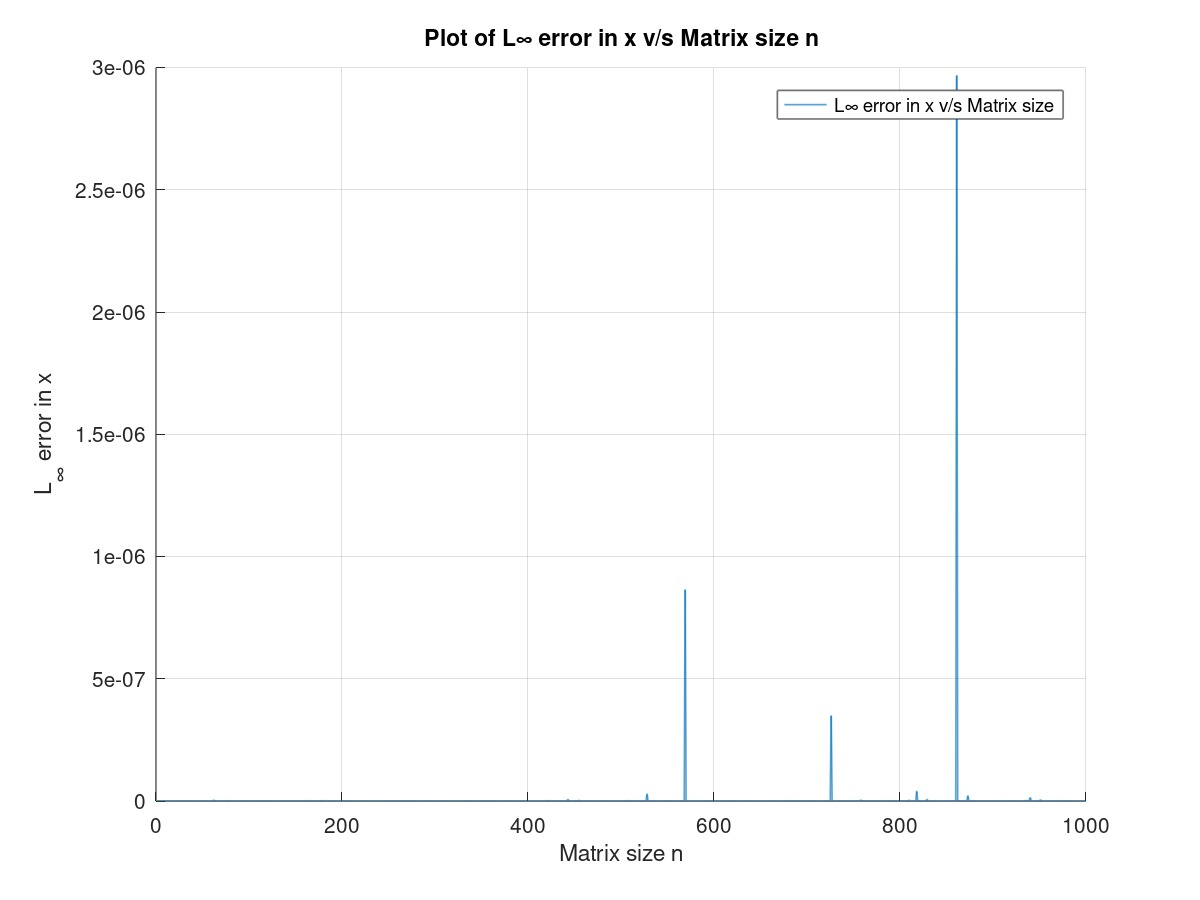
\includegraphics[scale=0.35]{Figure_1.jpeg}
		}
	\end{center}
	\caption{Plot of the L$\infty$ error in $x$ v/s Matrix Size  $\epsilon$ [1, 1000]}
\end{figure}
\section{Plot of Computational Time for $x$ v/s Matrix Size:}
In the following section I have represented the plot of the Computational Time for $x$ v/s Matrix Size  $\epsilon$ [1, 1000] while approximating the value of $x$ = $A^{-1}$ $b$ by using the four separate methods ie $QR$ Decomposition Method, Octave’s inbuilt $QR$ Decomposition Method, Inverse "$inv()$" Method, Backslash "$\backslash$" Method. The plot of the Computational Time for $x$ v/s Matrix size  $\epsilon$ [1, 1000] is shown below:
\clearpage
\begin{figure}[!ht]
	\begin{center}
		\framebox{
			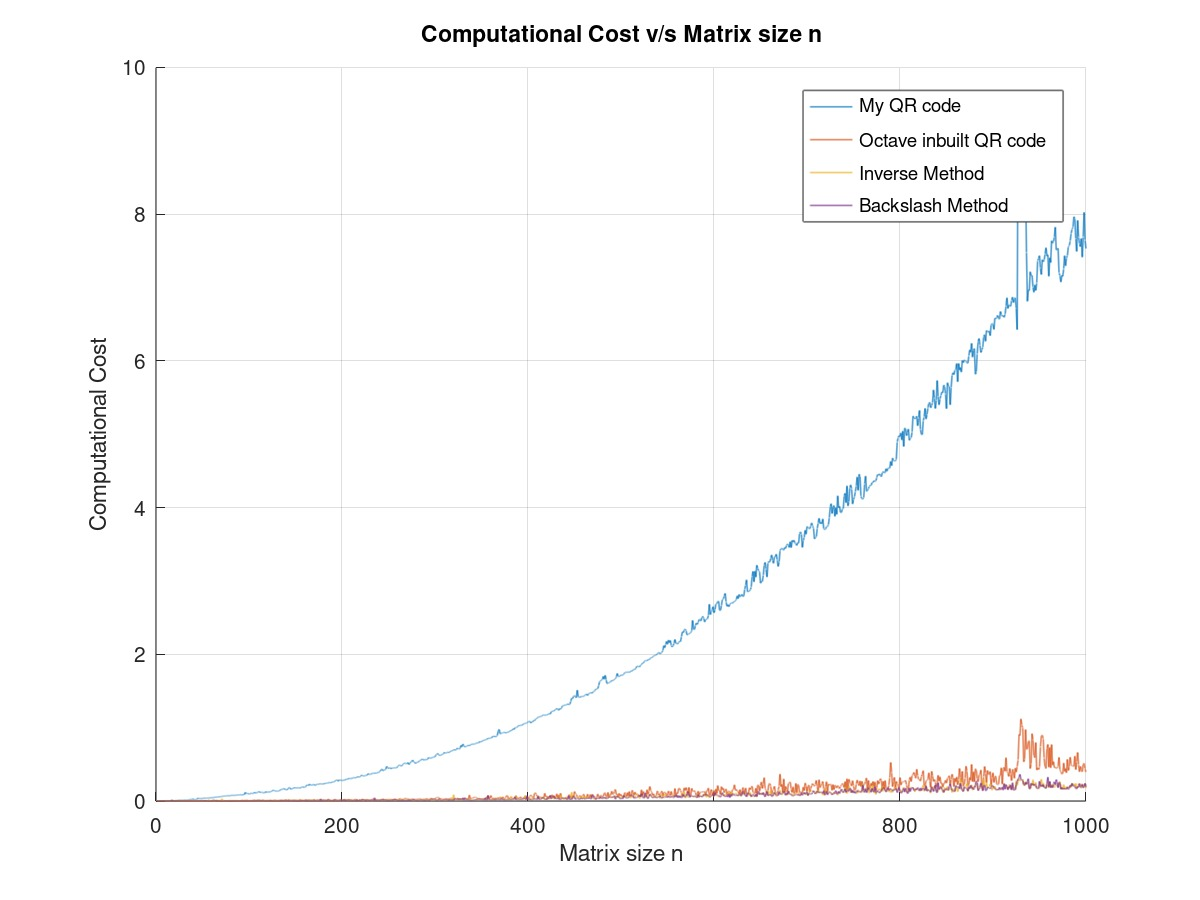
\includegraphics[scale=0.35]{Figure_2.jpeg}
		}
	\end{center}
	\caption{plot of the Computational Time for $x$ v/s Matrix Size  $\epsilon$ [1, 1000]}
\end{figure}
\bigskip
\section{Plot of Computational Time for $x$ v/s Matrix Size for my QR Method Code:}
In the following section I have represented the plot of the Computational Time for $x$ v/s Matrix Size  $\epsilon$ [1, 1000] while approximating the value of $x$ = $A^{-1}$ $b$ for the Total Computational Time, Time taken for generating Q and R, Time taken for the  Back-Substitution Method for solving $x$ against Matrix Size  $\epsilon$ [1, 1000]. The plot of the Computational Time for $x$ v/s Matrix Size  $\epsilon$ [1, 1000] while approximating the value of $x$ = $A^{-1}$ $b$ for the Total Computational Time, Time taken for generating Q and R, Time taken for the  Back-Substitution Method for solving $x$ against Matrix Size  $\epsilon$ [1, 1000] is shown below:
\clearpage
\begin{figure}[!ht]
	\begin{center}
		\framebox{
			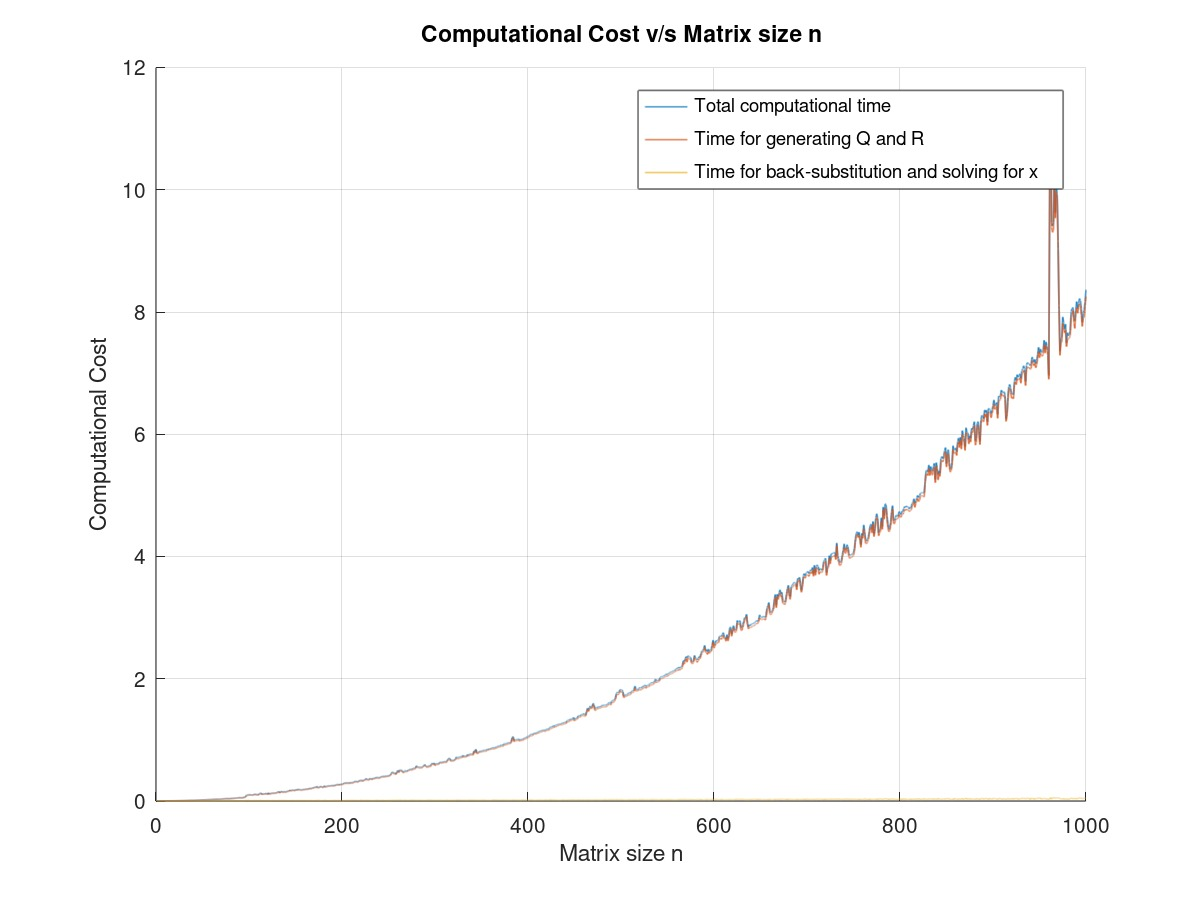
\includegraphics[scale=0.35]{Figure_3.jpeg}
		}
	\end{center}
	\caption{Plot of Computational Time for $x$ v/s Matrix Size for my QR Method Code}
\end{figure}
\end{document}
